\documentclass[10pt,conference,compsocconf]{IEEEtran}

\usepackage{hyperref}
\usepackage{graphicx}	% For figure environment
\usepackage{subfigure}
\usepackage{titling} % Customizing the title section
\usepackage{dblfloatfix}    % To enable figures at the bottom of page
\usepackage{kantlipsum}     % for random text
\usepackage{todonotes}
\usepackage[margin=0.9in]{geometry}

\begin{document}
	
\pretitle{\begin{center}\Huge\bfseries} % Article title formatting
\posttitle{\end{center}} % Article title closing formatting
\title{Deep Learning - Project 1}

\author{
	% Your name
	\textsc{Niccol\`{o} Sacchi, Succa Riccardo \& Marco Zoveralli}
	\normalsize{} \\
	% Your supervisors
	\textsc{Group:}
	\normalsize{RoadSegmentationFault}\\
	% Your institution
	\normalsize \'{E}cole polytechnique f\'{e}d\'{e}rale de Lausanne
}

\maketitle

\begin{abstract}
  The goal of this project is to train and test a predictor of finger movements (left or right hand) from Electroencephalography
(EEG) recordings. We decided to construct several solutions, starting from simple baseline models and then escalating to complex deep neural networks. 
\end{abstract}

\section{Introduction}
This project consists in a two-class classification problem to predict the laterality of incoming finger movements 130ms before key-press. The electical pulse that generates the finger movement starts a fraction of second before the actual movement, giving us the possibiliy to predict which hand the subject is going to move through an EEG analisys.


The following sections give an overview of the techniques that were tried in order to construct a predictor. Section~\ref{sec:data-analysis} breafly describes the dataset of EEG recondings and the experiment that was perfomed to obtain them; Section~\ref{sec:baselines} proposes a first approach to the problem by using a series of simple classification models (baselines); Section~\ref{sec:deep} goes to more complex solutions exploiting Fully Connected Neural Networks and Convolutional Neural Networks; Section~\ref{sec:results} compares the results obtained with the most performing models.



\section{Dataset}
\label{sec:data-analysis}
The dataset was provided by Fraunhofer-FIRST, Intelligent Data Analysis Group (Klaus-Robert Müller), and Freie Universität Berlin, Department of Neurology, Neurophysics Group. It was first given in the "BCI competition II" (May 2003) with a sample of 416 epochs, divided in 316 train records (labeled) and 100 test records (unlabeled).
The experiment perfomed to construct the dataset consisted in examining a normal subject sitting on a chair in a relaxed position, while he was typing on a computer keyboard in a self-chosen order. 3 sessions of 6 minutes each were taken, all conducted in the same day with a small break inbetween and with an average typing speed of 1 key/second. The EEG records were made by using 28 electodes to monitor the brain electrical activity. They measured a time slot of 500ms, ending 130ms before the keypress, and sampled at 100Hz and 1000Hz. 
In our project we used the records sampled at 100Hz, imported as a 28 (elecrode's measurements) x 50 (time frames) matrices. We also tested the 1000Hz records after we identified the best predictor model.
An example of a record with the respective label is shown in figure 1 -- Da mettere


\section{Baseline Models}
\label{sec:baseline}
All the baseline models were tested with cross-validation and we iterated over a range of values for some parameters in order to find the best score.
We implemented the following models (from sklearn library):\\
- Logistic Regression, tested with a grid search on the regularization parameter. Surprisingly, this model has good performance in our classification problem as shown in figure 2, despite the fact that it is much more simple than other models we tried.\\
- Random Forest Classifier, with iteration over the max depth of the trees.\\
- K-Nearest Neighbors, with multiple values for K. Moreover, before trainig this model, we normalized the input and applied a PCA to reduce the dimensions (we kept the 95\% of the signal energy)\\

\subsection{Baselines results} 
\begin{table*}
\begin{tabular}{ | c | c | }
\hline
Baseline & Test Accuracy  \\
\hline
\multirow{LogisticRegression}
& res1 \\
\hline
\multirow{Random Forest Classifier}
& res2 \\
\hline
\multirow{K-NN}
& res3 \\
\hline
\multirow{SVM}
& res4 \\
\hline
\multirow{Linear Discriminant Analysis}
& res5 \\
\hline
\end{tabular}
\end{table*}
The above table clearly shows that none among the well-known classifiers is really able to provide a proper solution to this problem. In the next section we show the improvements that were obtained through the adoption of our own model and the methodology behind its construction. 
\section{Deep Neural Networks}
\label{sec:deep}
We designed different models, starting from a Fully Connected Neural Network and then moving to Convolutional and Fully Concolutional Neural Networks. The increasing complexity of these models allowed us to get better perfomances on the test set, at the price of more time and resources needed.\\
Our methodology was based, at first, on building models that were inspired to the main concepts that were introduced during the lectures. Then, we focused on modifying these models with the goal of getting better results.
\subsection{Cross-validation}
One fundamental step of this approach consisted in adopting the cross-validation technique in order to extract the optimal parameters for each model. Given a certain parameter to optimize, the cross-validation technique consists, as first step, in splitting the available train dataset in k equal parts. Then, k-1 of these sets are used to train the model and 1 is used as a validation dataset. This process is repeated k times: at each iteration, a different part is considered as validation dataset and the remaining k-1 parts are considered as training dataset. This procedure must be repeated for a set of possible values that this parameter can assume. Finally, the parameter values that lead to the best prediction scores can be considered to be the optimal ones.
Two further considerations must be taken into account:\\
- There are a lot of parameters that influence the score. We considered some relevant ones: regularization terms, activation functions, optimizers, hidden units in the last layer. However, potentially relevant parameters are not considered during this optimization phase. For instance, we are not considering the filter dimensions, number of layers, the number of filters, etc. \\
- Getting the optimal combination of parameters implies enumerating all the possible combinations of all the parameters. This results in exponential complexity and, after some tries, we observed that this is unfeasible for our available computational resources. Therefore, we adopted an approximation of this methodology, which consisted in a greed approach in which we selected the optimal parameters singularly. Although this does not provide an optimal solution, it still provides some improvement and, more importantly, it allows to keep the algorithm complexity at an acceptable level (linear). \\

% cross-validation would work better if the dataset was bigger 
% hidden units in the last layer, optimizers (ADAM, adagrad, ..), activation functions, regularization terms


\section{Results}
\label{sec:results}

	The traditional CNN was trained for 1000 epochs, each consisting of 25 batches of 4 images, on a NVIDIA GeForce GTX graphics card with 2 GB of VRAM, obtaining an F1 score of 0.833. While the U-Net was trained for 10000 iteration with a learning rate $\lambda = 10^{-3}$ which lead to an F1 score of 0.9385 on the test set submitted on Kaggle.
	To compare different techniques we used the Precision Recall method (PR) which focuses on the relevance of the prediction on the labels of a test set. To compute the PR values we split the training dataset into two subsets, one used for training and one used to compute the PR curve. The latter is computed by gradually increasing the threshold (used to establish, given its probability, if a pixel is a road) to compute different PR values. By doing so, we obtain the graph in Figure \ref{fig:pr}.

	\begin{figure}[h]
		\centering
		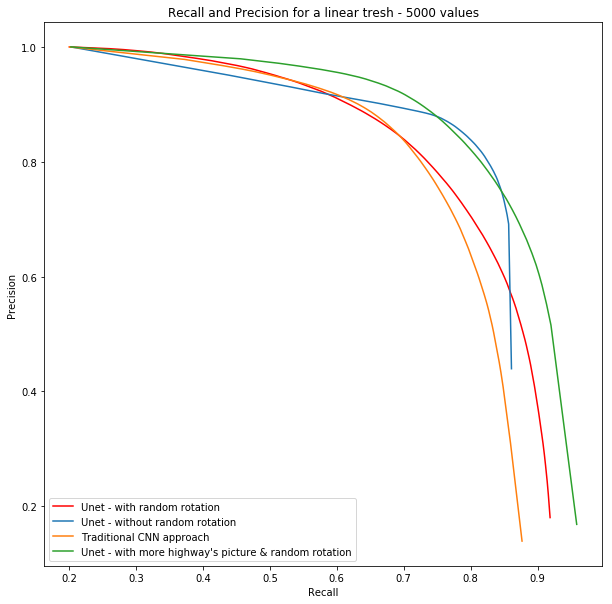
\includegraphics[width=0.8\columnwidth]{img/pr_curve.png}
		\caption{Precision and recall evolution regarding our different methods}
		\label{fig:pr}
	\end{figure}
	
	We can observe three important things in this plot. Since the yellow curve is below every others, we can say that Unet is perfroming better than the traditional approach. The second observation is that the green curve is above the red one. Considering this we can conclude that adding more highway images and getting rid of the seaside images was a good thing. The third observation is about the blue curve. We can see that in some cases the blue curve is above the green one. In fact when we are not rotating the image the network learns better how to detect vertical and horizontal lines but the results are worse when predicting the others. That explains why the blue curve goes above the yellow one between 0.6 and 0.8. We concluded that the yellow curve corresponds to the best model and therefore the one we used for the Kaggle competition.
	
\section{Conclusion}
\label{sec:conclusion}
Both models proved to be versatile and effective in achieving good predictions. However, our traditional CNN model failed in recognizing narrow roads, especially when they are covered by shadows, those types of roads are indeed almost inexistent in the training set while present in many images of the test set. Moreover, the train and test datasets were mainly restricted to cities. To obtain a model that would efficiently work with a wider range of input images such as images with snow, country images or on different meteorological conditions, we would require a bigger and diverse training set. In addition, without any preprocessing other than data augmentation, both models outperformed the baselines and confirmed their superiority in solving this kind of problem.


\bibliographystyle{IEEEtran}
\bibliography{groupRoadSegmentationFault-literature}

\end{document}
